\documentclass[
  11pt,
  letterpaper,
   addpoints,
   answers
  ]{exam}

\usepackage[utf8]{inputenc}
\usepackage{../exercise-preamble}
\usepackage{float}
\usepackage{subcaption}
% TikZ libraries needed for `right=.. of ..` and coordinate math
\usetikzlibrary{positioning,calc,arrows,arrows.meta}
% Alias de seguridad por si se escribe 'ikzstyle' por error
\let\ikzstyle\tikzstyle

\begin{document}

\noindent
\begin{minipage}{0.47\textwidth}

\includegraphics[width=\textwidth]{../fcfm_die}
\end{minipage}
\begin{minipage}{0.53\textwidth}
\begin{center} 
\large\textbf{Análisis de señales} (EL3203-2) \\
\large\textbf{Clase auxiliar 3} \\
\normalsize Prof.~Jorge Silva.\\
\normalsize Prof.~Aux.~Erik Sáez
\end{center}
\end{minipage}

\vspace{0.5cm}
\noindent
\vspace{.85cm}
%----------------------------
\noindent\rule{\textwidth}{0.4pt}
\subsection*{Serie de Fourier de una señal $T$-periódica}
La serie de Fourier permite descomponer cualquier señal periódica en una suma de funciones sinusoidales (armónicos) de distintas frecuencias, amplitudes y fases. Cada armónico tiene una frecuencia múltiplo de la fundamental $\omega_0=\tfrac{2\pi}{T}$, donde $T$ es el período de la señal. Así, cualquier señal $T$-periódica se puede escribir como:
\begin{equation}
  x(t) = \sum_{k=-\infty}^{\infty} c_k\,e^{jk\omega_0 t}
\end{equation}
Los coeficientes $c_k$ indican el peso (amplitud y fase) de cada armónico en la señal.

\subsubsection*{Base armónica y ortogonalidad}
Las funciones $\psi_k(t)=e^{jk\omega_0 t}$ forman una base ortogonal en el intervalo de un período. Esto significa que cada armónico es independiente de los demás y se puede calcular por separado:
\begin{equation}
  \frac{1}{T}\int_{t_0}^{t_0+T}\psi_k(t)\,\psi_m^{*}(t)\,dt = \begin{cases} 1,& k=m,\\ 0,& k\neq m. \end{cases}
\end{equation}
Esta propiedad facilita el cálculo de los coeficientes de Fourier.

\subsubsection*{Ecuaciones de análisis y síntesis}
	\textbf{Síntesis:} reconstruye la señal a partir de los coeficientes:
\begin{equation}
  x(t) = \sum_{k=-\infty}^{\infty} c_k\,e^{jk\omega_0 t}
\end{equation}
	\textbf{Análisis:} permite calcular cada coeficiente a partir de la señal:
\begin{equation}
  c_k = \frac{1}{T}\int_{t_0}^{t_0+T} x(t)\,e^{-jk\omega_0 t}\,dt
\end{equation}
El intervalo $[t_0, t_0+T]$ puede elegirse arbitrariamente, siempre que cubra un período completo.

\subsubsection*{Simetrías para señales reales}
Si la señal $x(t)$ es real, los coeficientes cumplen $c_{-k}=c_k^{*}$ (simetría conjugada), lo que implica que la magnitud es igual y la fase opuesta para $k$ y $-k$. Si la señal es par, sólo aparecen cosenos; si es impar, sólo senos.

\subsection*{Aproximación finita (truncada)}
En la práctica, se usan sólo los primeros $K$ armónicos para aproximar la señal:
\begin{equation}
  x_K(t) = \sum_{k=-K}^{K} c_k\,e^{jk\omega_0 t}
\end{equation}
Esto es útil para análisis numérico y simulaciones. Cerca de discontinuidades pueden aparecer oscilaciones (efecto Gibbs). El valor de $K$ depende de la precisión deseada y la naturaleza de la señal.

\begin{figure}[H]
  \centering
  \begin{subfigure}[t]{0.48\textwidth}
    \centering
    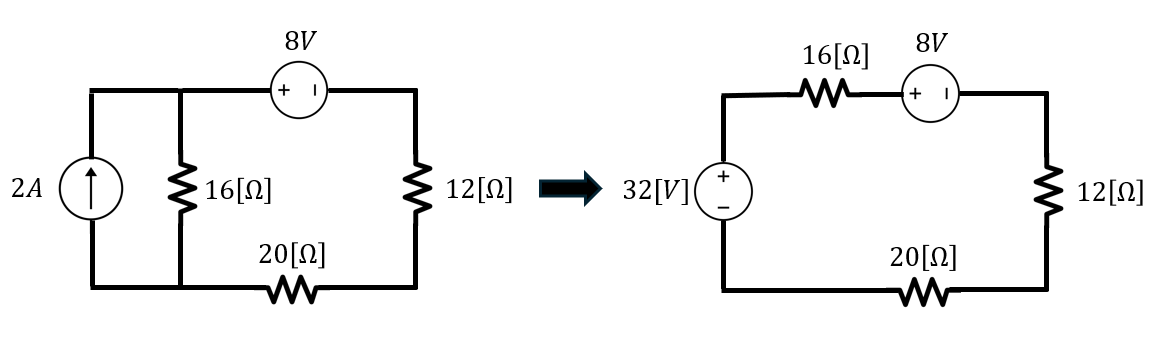
\includegraphics[width=\linewidth]{Auxiliar_3_6}
    \caption{Aproximación con $K=1$ armónico impar.}
  \end{subfigure}
  \hfill
  \begin{subfigure}[t]{0.48\textwidth}
    \centering
    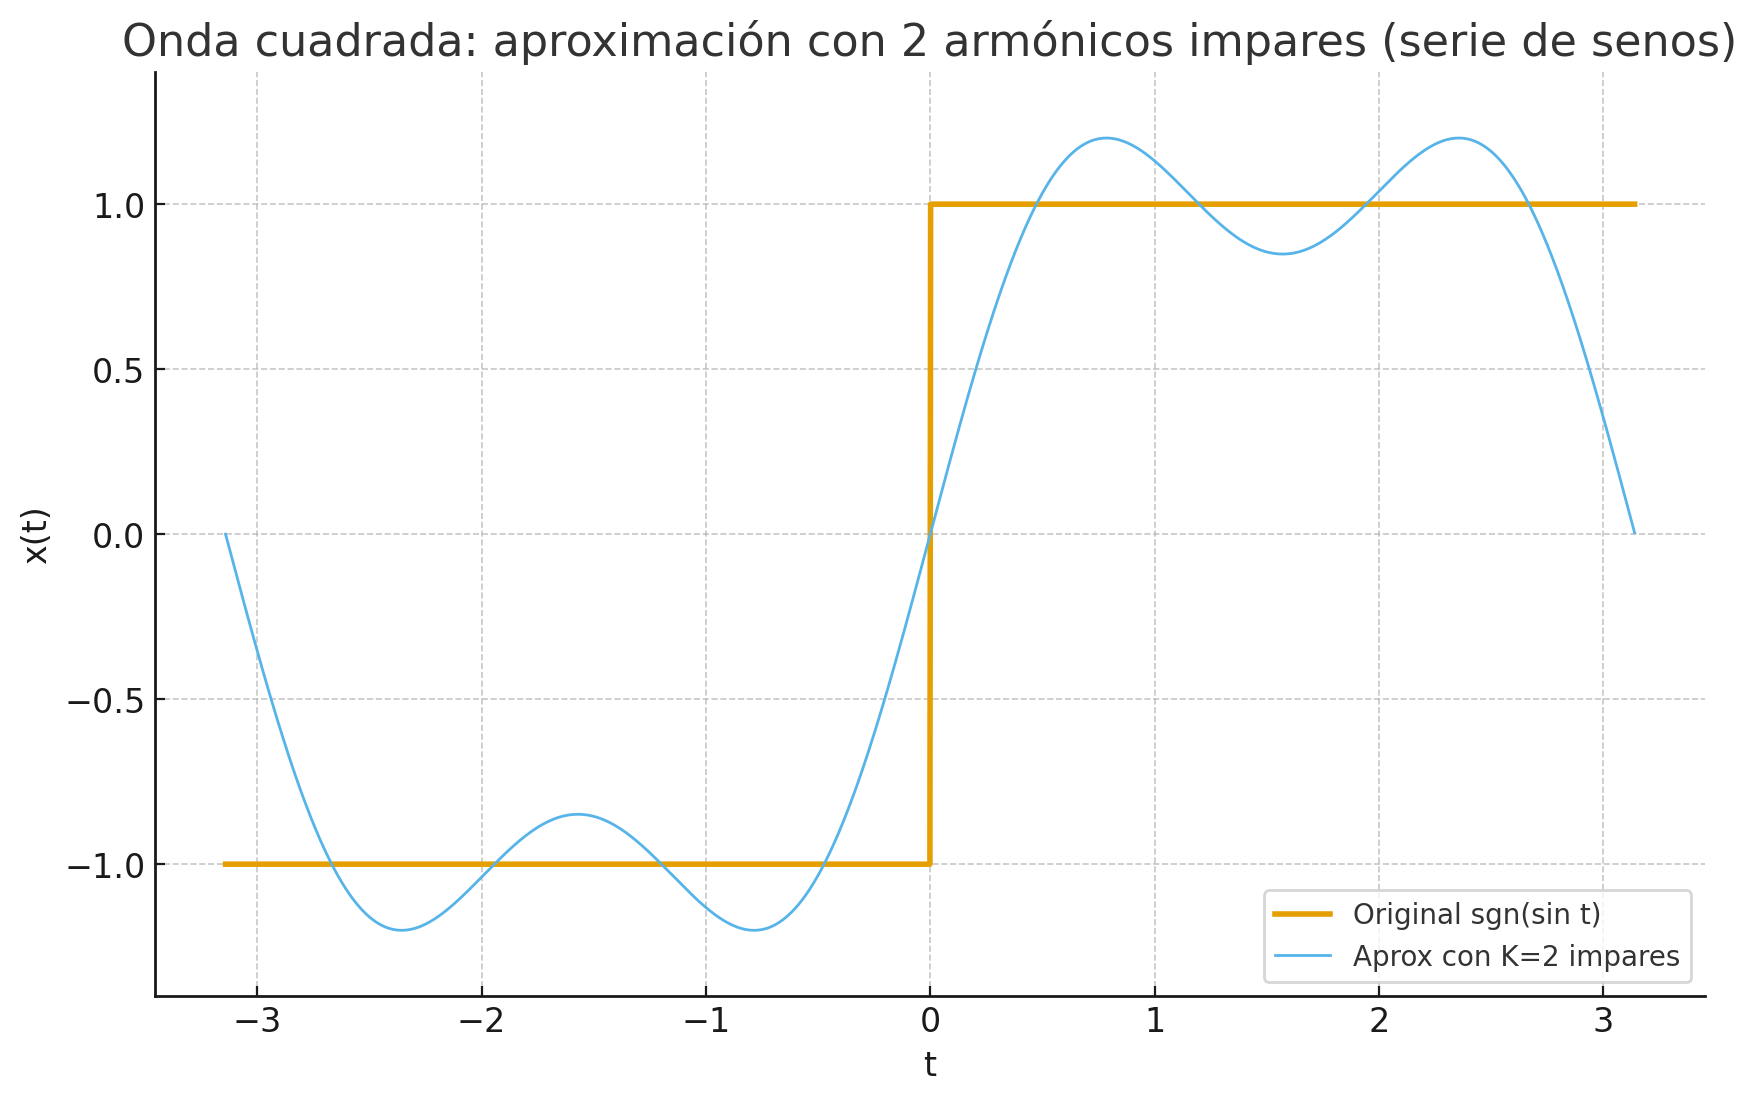
\includegraphics[width=\linewidth]{Auxiliar_3_7}
    \caption{Aproximación con $K=2$ armónicos impares.}
  \end{subfigure}
    
  \begin{subfigure}[t]{0.48\textwidth}
    \centering
    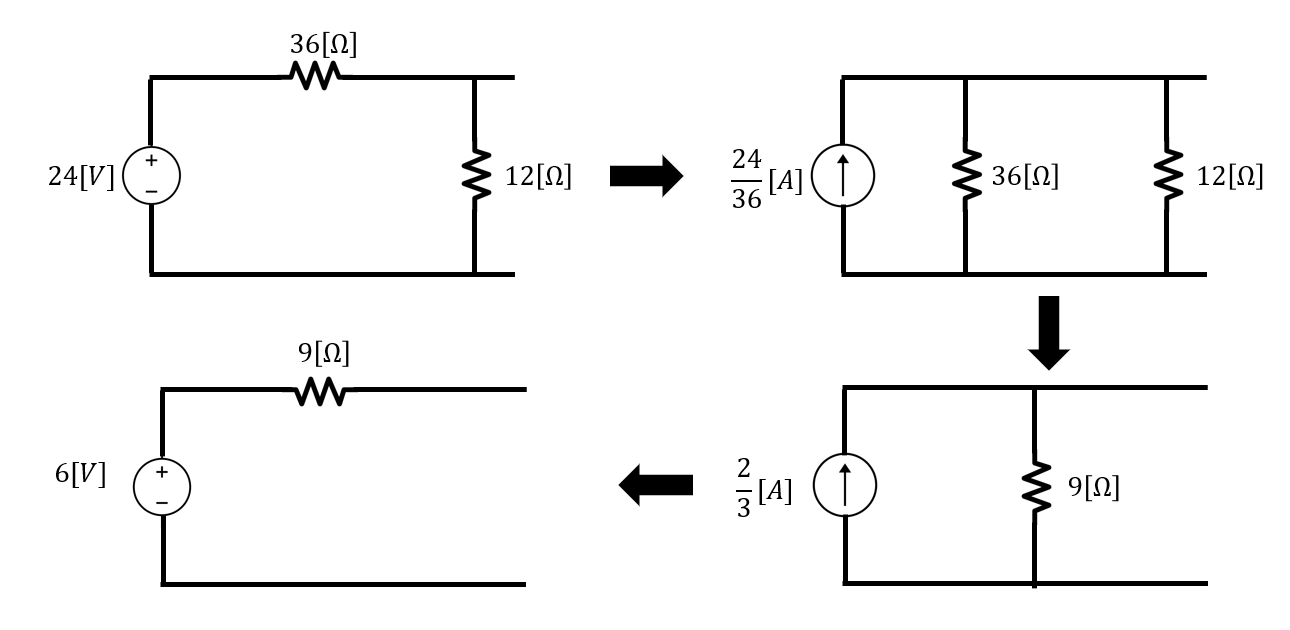
\includegraphics[width=\linewidth]{Auxiliar_3_8}
    \caption{Aproximación con $K=5$ armónicos impares.}
  \end{subfigure}
  \hfill
  \begin{subfigure}[t]{0.48\textwidth}
    \centering
    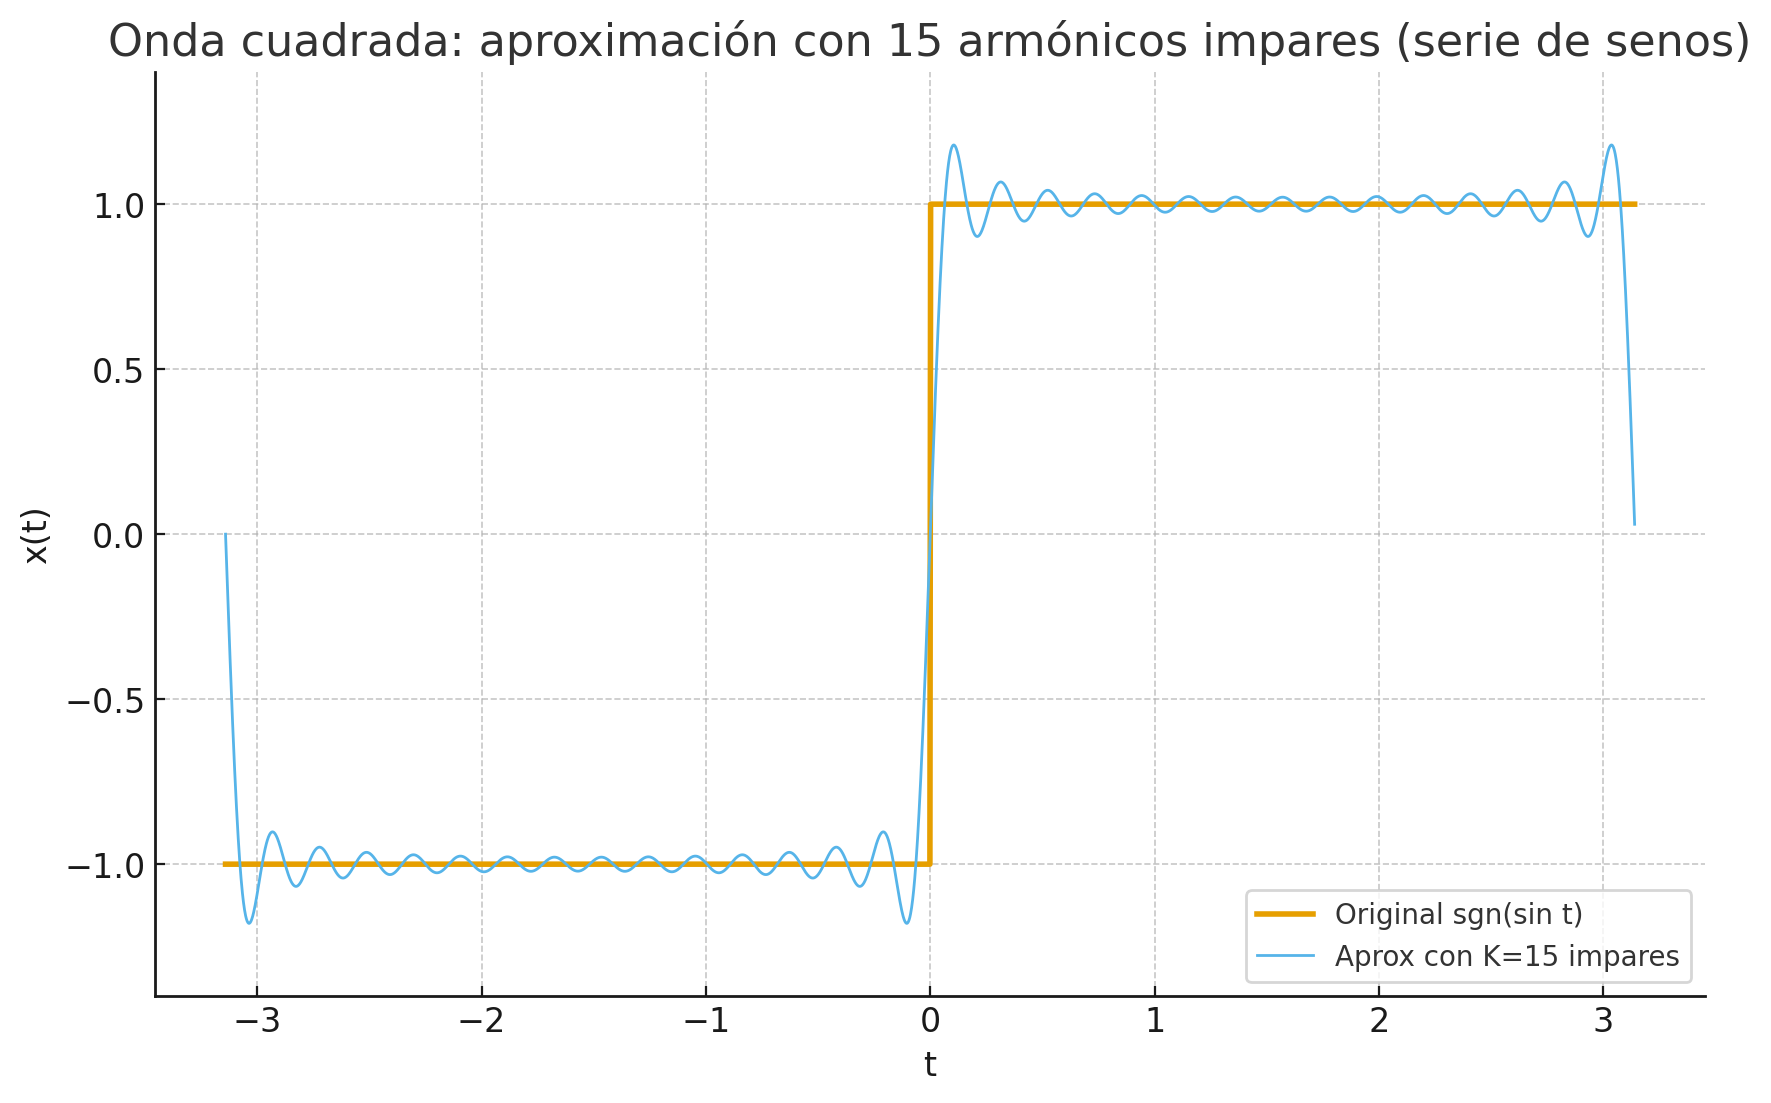
\includegraphics[width=\linewidth]{Auxiliar_3_9}
    \caption{Aproximación con $K=15$ armónicos impares.}
  \end{subfigure}
  \caption{Aproximación de una onda cuadrada mediante la suma de los primeros $K$ armónicos impares (serie de senos). Se observa cómo la aproximación mejora al aumentar $K$, pero aparecen oscilaciones cerca de las discontinuidades (efecto Gibbs).}
  \label{fig:aprox_cuadrada}
\end{figure}

\subsection*{Energía y potencia}
La energía de una señal mide el "contenido total" a lo largo del tiempo:
\begin{equation}
  E_x = \int_{-\infty}^{\infty} |x(t)|^2\,dt
\end{equation}
Para señales periódicas, la energía es infinita, pero se define la potencia promedio en un período:
\begin{equation}
  P_x = \frac{1}{T}\int_{t_0}^{t_0+T} |x(t)|^2\,dt
\end{equation}
La potencia indica cuánta energía se transfiere en promedio por unidad de tiempo.

\subsection*{Relación de Parseval (señales periódicas)}
La relación de Parseval conecta el dominio temporal y el de frecuencias:
\begin{equation}
  P_x = \frac{1}{T}\int_{t_0}^{t_0+T} |x(t)|^2\,dt = \sum_{k=-\infty}^{\infty} |c_k|^2
\end{equation}
Esto permite calcular la potencia directamente a partir de los coeficientes de Fourier, sin necesidad de integrar en el tiempo.\\
\noindent\rule{\textwidth}{0.4pt}
\newpage
%----------------------------
\begin{questions}
%----------------------------
\question
Considere la familia de funciones exponenciales discretas:
\begin{equation}
  A = \left\{ (\gamma_a(n)) \in \mathbb{R}^{\mathbb{N}} : \gamma_a(n) = a^n u(n),\ 0 < a < 1 \right\}
\end{equation}
\begin{enumerate}
  \item Verifique que el impulso discreto $\delta(n)$ puede ser expresado punto a punto como:
  \begin{equation}
    \delta(n) = \gamma_a(n) - a\,\gamma_a(n-1)
  \end{equation}
  \item Del punto anterior, muestre que toda señal discreta $x(n) \in \mathbb{R}^{\mathbb{Z}}$ puede ser descompuesta como:
  \begin{equation}
    x(n) = \sum_{k=-\infty}^{\infty} c_k\,\gamma_a(n-k)
  \end{equation}
  \item Use las propiedades de linealidad e invariancia en el tiempo para expresar la salida $y(n) = \mathcal{T}[x(n)]$ en términos de la entrada $x(n)$ y la señal $g(n) = \mathcal{T}[\gamma_a(n)]$.
\end{enumerate}
%----------------------------
\begin{solution}
\subsection*{Resolución 1.1}
Sea la familia de funciones exponenciales discretas:
\begin{equation}
A = \Big\{ \gamma_a(n) \in \mathbb{R}^{\mathbb{N}} : \gamma_a(n) = a^n u(n), \; 0<a<1 \Big\}.
\end{equation}

Queremos verificar que:
\begin{equation}
\delta(n) = \gamma_a(n) - a\,\gamma_a(n-1).
\end{equation}

Dado que se busca demostrar lo anterior, tendremos lo siguiente:
\begin{align}
\gamma_a(n) - a\,\gamma_a(n-1) &= a^n u(n) - a\cdot a^{n-1}u(n-1) \\
&= a^n u(n) - a^n u(n-1) \\
&= a^n\big[u(n) - u(n-1)\big].
\end{align}

Recordemos que:
\begin{equation}
u(n) - u(n-1) =
\begin{cases}
1, & n=0, \\
0, & n\neq 0,
\end{cases}
\end{equation}
lo cual corresponde exactamente a la definición del impulso discreto \(\delta(n)\). Por lo tanto:
\begin{equation}
\delta(n) = \gamma_a(n) - a\,\gamma_a(n-1).
\end{equation}

\subsection*{Resolución 1.2}
Sabemos que cualquier señal discreta \(x(n)\) puede expresarse como:
\begin{equation}
x(n) = \sum_{k \in \mathbb{Z}} x(k)\,\delta(n-k).
\end{equation}

Sustituyendo la expresión de \(\delta(n)\) obtenida en el punto anterior:
\begin{align}
x(n) &= \sum_{k \in \mathbb{Z}} x(k)\Big[ \gamma_a(n-k) - a\,\gamma_a(n-k-1)\Big] \\
&= \sum_{k \in \mathbb{Z}} x(k)\,\gamma_a(n-k) \;-\; a \sum_{k \in \mathbb{Z}} x(k)\,\gamma_a(n-k-1).
\end{align}

En la segunda suma hacemos el cambio de variable \(k \mapsto k-1\):
\begin{equation}
\sum_{k \in \mathbb{Z}} x(k)\,\gamma_a(n-k-1) 
= \sum_{k \in \mathbb{Z}} x(k-1)\,\gamma_a(n-k).
\end{equation}

Por tanto:
\begin{align}
x(n) &= \sum_{k \in \mathbb{Z}} \Big[x(k) - a\,x(k-1)\Big] \,\gamma_a(n-k).
\end{align}

Definiendo:
\begin{equation}
c_k = x(k) - a\,x(k-1),
\end{equation}
tenemos finalmente:
\begin{equation}
x(n) = \sum_{k \in \mathbb{Z}} c_k\,\gamma_a(n-k).
\end{equation}

\subsection*{Resolución 1.3}
Sea el sistema \( \mathcal{T} \) lineal e invariante en el tiempo (LTI). Definimos:
\begin{equation}
g(n) = \mathcal{T}[\gamma_a(n)].
\end{equation}

La respuesta al impulso del sistema es:
\begin{equation}
h(n) = \mathcal{T}[\delta(n)].
\end{equation}

Usando el resultado de 1.1:
\begin{align}
h(n) &= \mathcal{T}\big[\gamma_a(n) - a\,\gamma_a(n-1)\big] \\
&= \mathcal{T}[\gamma_a(n)] - a\,\mathcal{T}[\gamma_a(n-1)] \\
&= g(n) - a\,g(n-1).
\end{align}

Finalmente, como el sistema es LTI:
\begin{align}
y(n) &= (x * h)(n) \\
&= \sum_{k \in \mathbb{Z}} x(k)\,h(n-k) \\
&= \sum_{k \in \mathbb{Z}} x(k)\Big[g(n-k) - a\,g(n-k-1)\Big].
\end{align}

De este modo:
\begin{equation}
y(n) = \sum_{k \in \mathbb{Z}} x(k)\,\big[g(n-k) - a\,g(n-k-1)\big].
\end{equation}

\end{solution}

%----------------------------
\question
\begin{enumerate}
  \item Determine la transformada de Fourier de las siguientes señales y gráfiquela en magnitud y fase:
\begin{align*}
  &\bullet\quad x(t) = \begin{cases}
    A \cdot e^{-a t} & t \geq 0 \\
    0 & t < 0
  \end{cases} \\
  &\bullet\quad x(t) = A \cdot e^{-a|t|}
\end{align*}

\item Determine los coeficientes de la serie de Fourier para la siguiente señal:
\begin{equation}
  x(t) = 1 + \sin(\omega_0 t) + 2\cos(\omega_0 t) + \cos\left(2\omega_0 t + \frac{\pi}{4}\right)
\end{equation}
\end{enumerate}
%----------------------------
\begin{solution}
\subsection*{Resolución 2.1}
Se pide la transformada de Fourier de las funciones dadas, luego por definición:
\begin{align}
  X(F) &= \int_{-\infty}^{\infty} x(t)\,e^{-j2\pi F t}\,dt
\end{align}
Luego se tiene que la primera función se puede expresar en funcion del escalón unitario \(u(t)\):
\[
x(t)=A\,e^{-a t}\,u(t),\qquad a>0.
\]
Por definición,
\begin{align}
X(F)
  &= \int_{-\infty}^{\infty} x(t)\,e^{-j2\pi F t}\,dt \\
  &= \int_{0}^{\infty} A e^{-a t}\,e^{-j2\pi F t}\,dt \\
  &= A\int_{0}^{\infty} e^{-(a+j2\pi F)t}\,dt \\
  &= A\left[\frac{-1}{a+j2\pi F}\,e^{-(a+j2\pi F)t}\right]_{0}^{\infty} \\
  &= \frac{A}{a+j2\pi F}.
\end{align}

Luego tenemos que el modulo y fase vienen dados por:
\begin{align}
|X(F)|
  &= \frac{A}{\sqrt{a^{2}+(2\pi F)^{2}}},\\
\angle X(F)
  &= \angle\big((a+j2\pi F)^{-1}\big)
   = -\arctan\!\left(\frac{2\pi F}{a}\right),
\end{align}
Luego gráficamente tenemos que: 

\begin{figure}[H]
  \centering

  \begin{subfigure}[t]{0.48\textwidth}
    \centering
    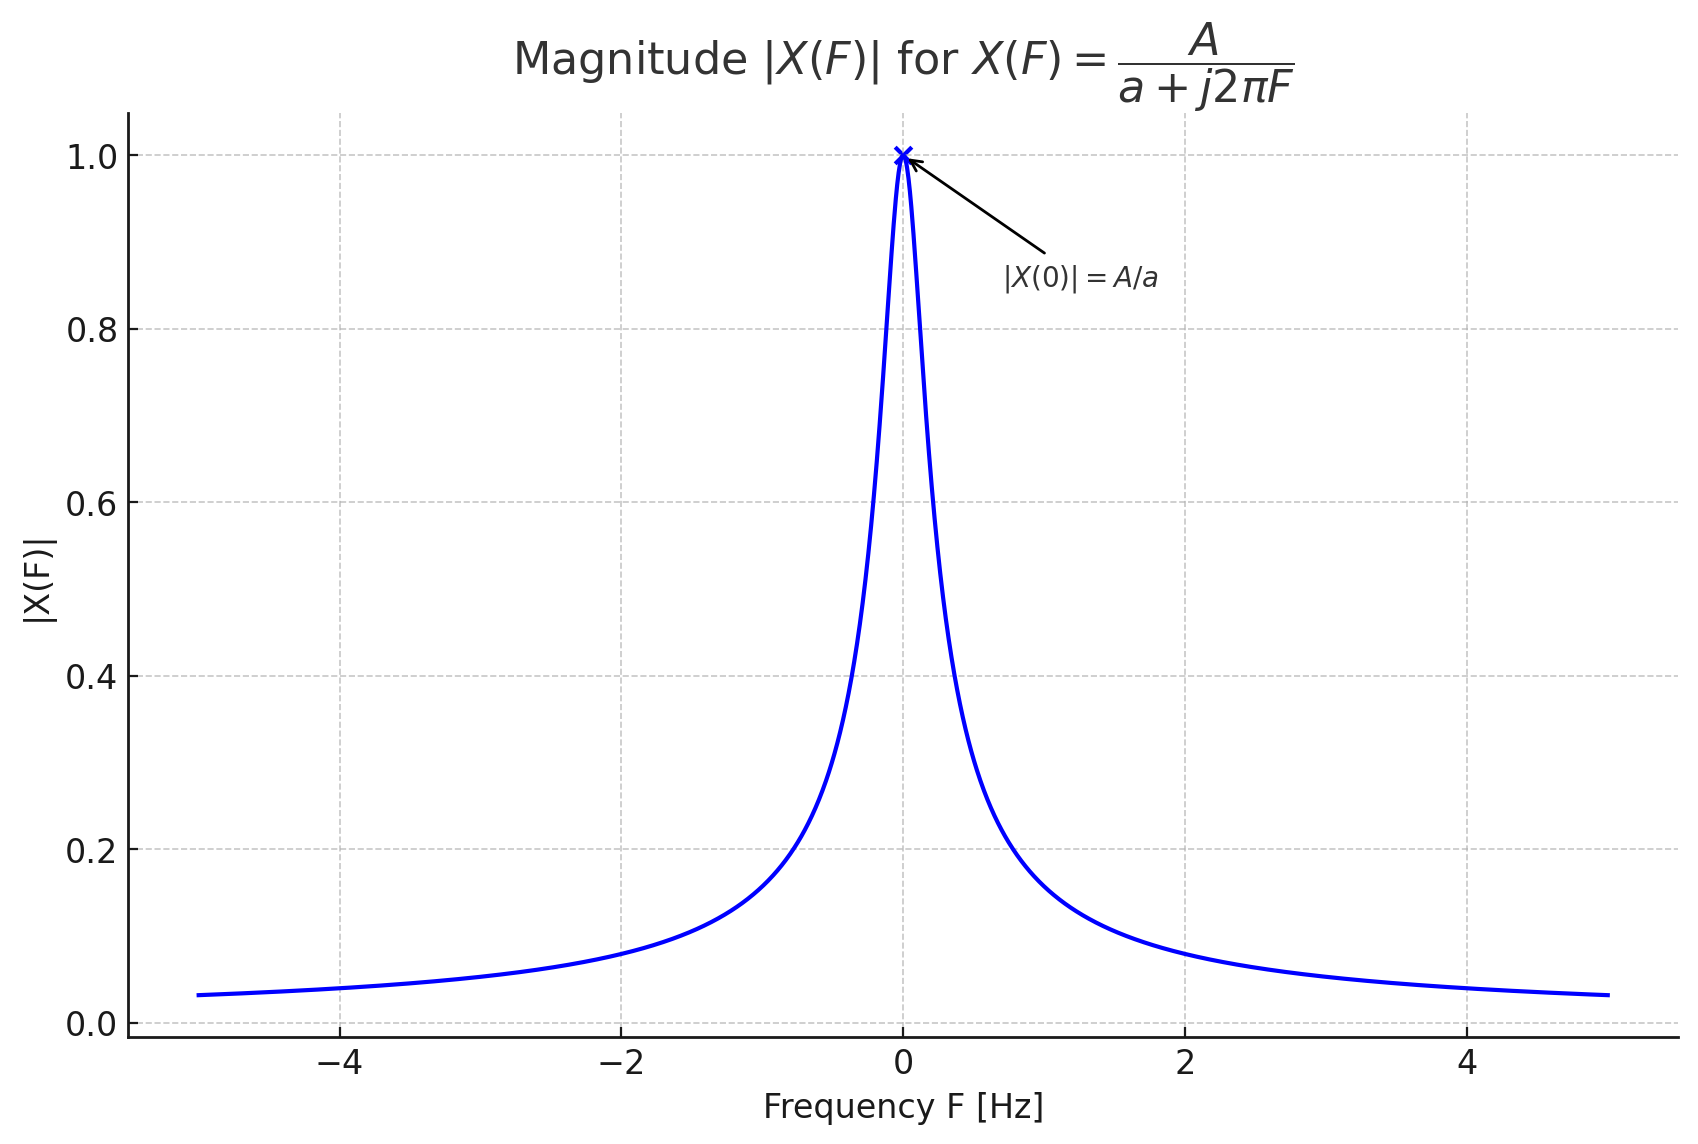
\includegraphics[width=1\linewidth]{Auxiliar_3_2} % <-- pon la extensión si hace falta
    \caption{Magnitud $|X(F)|$ para $X(F)=\frac{A}{a+j2\pi F}$. Se observa un máximo en $F=0$ igual a $A/a$, y la magnitud decae rápidamente para frecuencias altas, mostrando el comportamiento típico de un filtro pasabajo exponencial.}
    \label{fig:mag_XF}
  \end{subfigure}
  \hfill
  \begin{subfigure}[t]{0.48\textwidth}
    \centering
    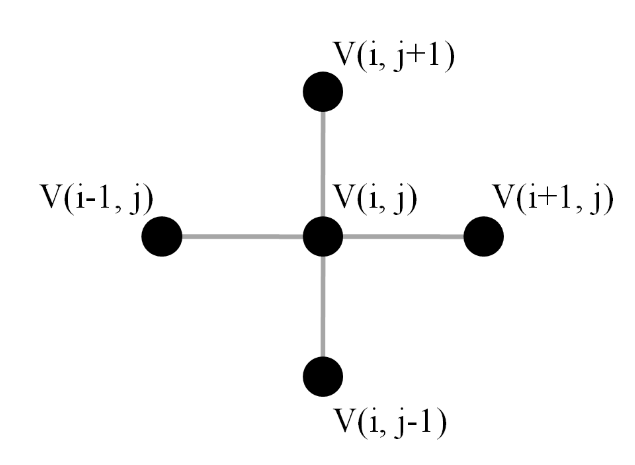
\includegraphics[width=1\linewidth]{Auxiliar_3_3}
    \caption{Fase $\angle X(F)$ para $X(F)=\frac{A}{a+j2\pi F}$. La fase parte en $0$ para $F=0$ y varía suavemente desde $+\pi/2$ a $-\pi/2$ al aumentar $|F|$, indicando el retardo de fase introducido por el sistema.}
    \label{fig:fase_XF}
  \end{subfigure}

  \caption{Magnitud y fase de la transformada de Fourier para $x(t)=A e^{-a t}u(t)$. La magnitud tiene máximo en $F=0$ y la fase varía de $+\pi/2$ a $-\pi/2$ según la frecuencia, mostrando el efecto de la exponencial sobre el espectro.}
  \label{fig:mag_fase_XF}
\end{figure}


Sea ahora la siguiente funcion:
\[
x(t)=A\,e^{-a|t|},\qquad a>0,
\]
que es par. Separando para \(t\ge 0\) y \(t<0\),
\begin{align}
X(F)
 &= \int_{-\infty}^{\infty} A e^{-a|t|} e^{-j2\pi F t}\,dt \\
 &= \int_{-\infty}^{0} A e^{+a t} e^{-j2\pi F t}\,dt
   + \int_{0}^{\infty} A e^{-a t} e^{-j2\pi F t}\,dt \\
 &= A\int_{-\infty}^{0} e^{(a-j2\pi F)t}\,dt
   +A\int_{0}^{\infty} e^{-(a+j2\pi F)t}\,dt \\
 &= A\left[\frac{1}{a-j2\pi F}e^{(a-j2\pi F)t}\right]_{-\infty}^{0}
   +A\left[\frac{-1}{a+j2\pi F}e^{-(a+j2\pi F)t}\right]_{0}^{\infty} \\
 &= \frac{A}{a-j2\pi F}+\frac{A}{a+j2\pi F}
  = \frac{A\big((a+j2\pi F)+(a-j2\pi F)\big)}{a^{2}+(2\pi F)^{2}} \\
 &= \frac{2A a}{a^{2}+(2\pi F)^{2}}.
\end{align}

Como \(x(t)\) es par, \(X(F)\) es real y par:
\begin{align}
|X(F)|
  &= \frac{2A a}{a^{2}+(2\pi F)^{2}},\\
\angle X(F)
  &= 0\quad \text{(para todo \(F\), salvo el signo en \(F\) donde \(X(F)>0\))}.
\end{align}
Luego gráficamente tenemos lo siguiente:
\begin{figure}[H]
  \centering

  \begin{subfigure}[t]{0.48\textwidth}
    \centering
    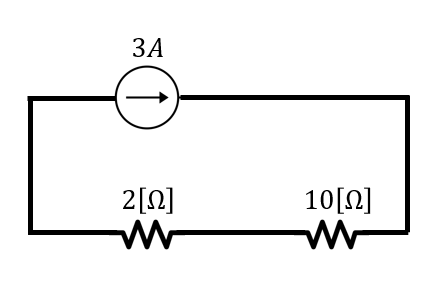
\includegraphics[width=1\linewidth]{Auxiliar_3_4} % <-- pon la extensión si hace falta
    \caption{Magnitud $|X(F)|$ para $X(F)=\frac{2Aa}{a^2+(2\pi F)^2}$. Se observa un máximo en $F=0$ igual a $2A/a$, y la magnitud es real, par y decae para frecuencias altas, mostrando el espectro de una exponencial simétrica.}
    \label{fig:mag_XF}
  \end{subfigure}
  \hfill
  \begin{subfigure}[t]{0.48\textwidth}
    \centering
    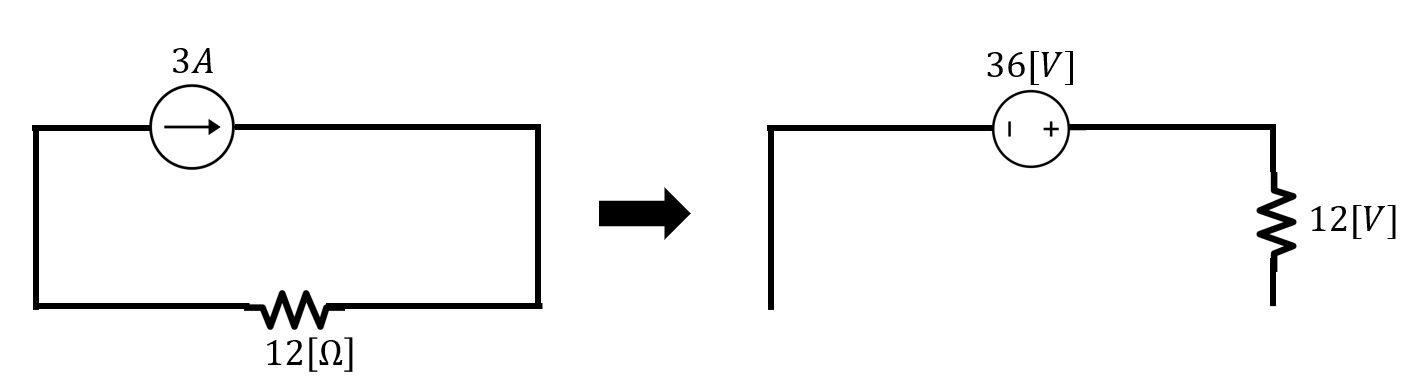
\includegraphics[width=1\linewidth]{Auxiliar_3_5}
    \caption{Fase $\angle X(F)$ para $X(F)=\frac{2Aa}{a^2+(2\pi F)^2}$. La fase es cero para todo $F$, lo que indica que la señal original es par y su transformada es completamente real.}
    \label{fig:fase_XF2}
  \end{subfigure}

  \caption{Magnitud y fase de la transformada de Fourier para $x(t)=A e^{-a|t|}$. La magnitud es real y par, con máximo en $F=0$, y la fase es cero en todo el dominio de frecuencias.}
  \label{fig:mag_fase_XF2}
\end{figure}

\subsection*{Resolución 2.2}
Los coeficientes de la serie de Fourier \( \{c_k\}_{k\in\mathbb{Z}} \) permiten expresar una señal periódica como combinación lineal de sinusoides complejas. En la forma compleja,
\begin{equation}
x(t)=\sum_{k=-\infty}^{\infty} c_k\,e^{jk\omega_0 t}, 
\qquad \omega_0=\frac{2\pi}{T},
\end{equation}
donde \(T\) es el período fundamental. Los coeficientes se obtienen (sobre cualquier intervalo de longitud \(T\)) como
\begin{equation}
c_k=\frac{1}{T}\int_{t_0}^{t_0+T} x(t)\,e^{-jk\omega_0 t}\,dt .
\end{equation}
Para convertir senos y cosenos a exponenciales usamos las identidades de Euler:
\begin{align}
\cos(\theta) &= \frac{e^{j\theta}+e^{-j\theta}}{2}, &
\sin(\theta) &= \frac{e^{j\theta}-e^{-j\theta}}{2j}.
\end{align}

Dada la señal
\begin{equation}
x(t)=1+\sin(\omega_0 t)+2\cos(\omega_0 t)+\cos\!\left(2\omega_0 t+\frac{\pi}{4}\right),
\end{equation}
la escribimos en forma exponencial y agrupamos por armónicos \(e^{jk\omega_0 t}\):
\begin{align}
x(t)
&= 1
+ \frac{1}{2j}e^{j\omega_0 t}-\frac{1}{2j}e^{-j\omega_0 t}
+ \left(e^{j\omega_0 t}+e^{-j\omega_0 t}\right)
+ \frac{1}{2}e^{j\frac{\pi}{4}}e^{j2\omega_0 t}
+ \frac{1}{2}e^{-j\frac{\pi}{4}}e^{-j2\omega_0 t} \\
&= 1
+ \Big(1+\tfrac{1}{2j}\Big)e^{j\omega_0 t}
+ \Big(1-\tfrac{1}{2j}\Big)e^{-j\omega_0 t}
+ \frac{1}{2}e^{j\frac{\pi}{4}}e^{j2\omega_0 t}
+ \frac{1}{2}e^{-j\frac{\pi}{4}}e^{-j2\omega_0 t}.
\end{align}
Identificando término a término con \(x(t)=\sum_k c_k e^{jk\omega_0 t}\), los coeficientes complejos son:
\begin{align}
c_0 &= 1, \\
c_{1} &= 1+\frac{1}{2j}=1-\frac{j}{2}, \\
c_{-1} &= 1-\frac{1}{2j}=1+\frac{j}{2}, \\
c_{2} &= \frac{1}{2}e^{j\frac{\pi}{4}}=\frac{\sqrt{2}}{4}(1+j), \\
c_{-2} &= \frac{1}{2}e^{-j\frac{\pi}{4}}=\frac{\sqrt{2}}{4}(1-j), \\
c_k &= 0 \quad \text{para } |k|\ge 3.
\end{align}
Obsérvese que, al ser \(x(t)\) real, se cumple la simetría conjugada \(c_{-k}=c_k^{*}\).


\end{solution}

%----------------------------
\question Para la función sinusoidal rectificada mostrada en la figura \ref{fig:aux3_1}, calcule los coeficientes de la serie de Fourier , ademas verifique el cumplimiento del teorema de Parseval.
\begin{figure}[H]
    \centering
    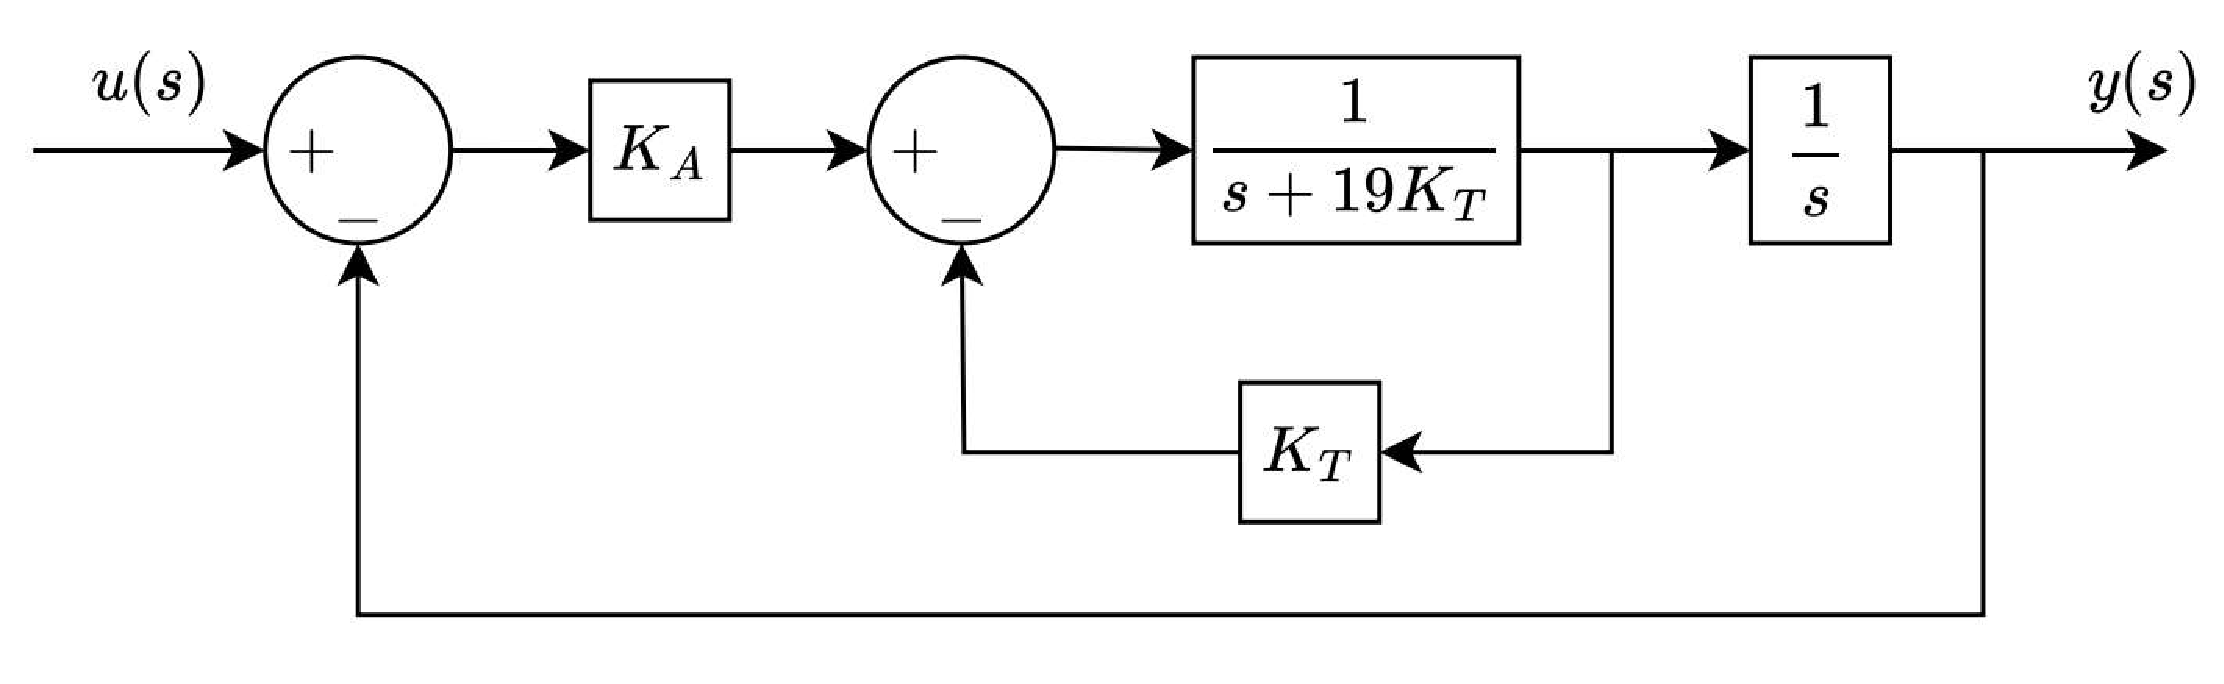
\includegraphics[width=0.6\textwidth]{Auxiliar_3_1}
    \caption{Función sinusoidal rectificada}
    \label{fig:aux3_1}
\end{figure}
%----------------------------
\begin{solution}
  \subsection*{Resolución 3.1}

Sea la sinusoidal rectificada de período \(\tau\) (se extiende periódicamente):
\begin{equation}
x(t)=A\,\sin\!\left(\frac{\pi t}{\tau}\right),\qquad 0\le t<\tau,
\end{equation}
con frecuencia fundamental \(f_0=\tfrac{1}{\tau}\) y pulsación \(\omega_0=\tfrac{2\pi}{\tau}\).
Los coeficientes complejos de Fourier se obtienen con la ecuación de análisis:
\begin{equation}
c_k=\frac{1}{\tau}\int_{0}^{\tau} x(t)\,e^{-jk\omega_0 t}\,dt.
\end{equation}
Sustituyendo \(x(t)\) y usando las identidades de Euler,
\(\sin\theta=\tfrac{e^{j\theta}-e^{-j\theta}}{2j}\), resulta
\begin{align}
c_k
&=\frac{A}{\tau}\int_{0}^{\tau}\sin\!\left(\frac{\pi t}{\tau}\right)e^{-j\frac{2\pi}{\tau}kt}\,dt\\
&=\frac{A}{2j\,\tau}\int_{0}^{\tau}\Big(e^{\,j\frac{\pi}{\tau}(1-2k)t}-e^{-\,j\frac{\pi}{\tau}(1+2k)t}\Big)\,dt\\
&=\frac{A}{2j\,\tau}\left[
\frac{e^{\,j\frac{\pi}{\tau}(1-2k)t}}{j\frac{\pi}{\tau}(1-2k)}
-\frac{e^{-\,j\frac{\pi}{\tau}(1+2k)t}}{-j\frac{\pi}{\tau}(1+2k)}
\right]_{0}^{\tau}.
\end{align}
Como \(e^{j\pi(1-2k)}=e^{-j\pi(1+2k)}=-1\) para todo \(k\in\mathbb{Z}\),
\begin{align}
c_k
&=\frac{A}{2j\,\tau}\left[
\frac{-2}{j\frac{\pi}{\tau}(1-2k)}+\frac{-2}{j\frac{\pi}{\tau}(1+2k)}
\right]
=\frac{A}{\pi}\left(\frac{1}{1-2k}+\frac{1}{1+2k}\right)\\
&=\frac{A}{\pi}\,\frac{(1+2k)+(1-2k)}{1-4k^2}
=\boxed{\;\frac{2A}{\pi\,(1-4k^2)}\;}.
\end{align}
En particular,
\begin{equation}
c_0=\frac{2A}{\pi},\qquad c_{-k}=c_k\quad(\text{coeficientes reales y pares}).
\end{equation}
Por otro lado buscamos realizar la verificacion de Parseval, por lo que la potencia promedio en el tiempo es
\begin{align}
P_x
=\frac{1}{\tau}\int_{0}^{\tau}x^2(t)\,dt
=\frac{A^2}{\tau}\int_{0}^{\tau}\sin^2\!\left(\frac{\pi t}{\tau}\right)\,dt
=\frac{A^2}{2}.
\end{align}
En frecuencia,
\begin{align}
\sum_{k=-\infty}^{\infty}|c_k|^2
=\frac{4A^2}{\pi^2}\sum_{k=-\infty}^{\infty}\frac{1}{(1-4k^2)^2}
=\frac{4A^2}{\pi^2}\!\left[\,1+2\sum_{k=1}^{\infty}\frac{1}{(1-4k^2)^2}\right].
\end{align}
Usando la identidad
\begin{equation}
\sum_{k=1}^{\infty}\frac{1}{(1-4k^2)^2}
=\frac{\pi^2}{16}-\frac{1}{2},
\end{equation}
se obtiene
\begin{align}
\sum_{k=-\infty}^{\infty}|c_k|^2
&=\frac{4A^2}{\pi^2}\left[\,1+2\!\left(\frac{\pi^2}{16}-\frac{1}{2}\right)\right]
=\frac{4A^2}{\pi^2}\cdot\frac{\pi^2}{8}
=\frac{A^2}{2}
=P_x,
\end{align}
con lo que queda verificada la relación de Parseval.
\end{solution}
%----------------------------
\question Dadas dos señales $f(t)$ y $g(t)$ con coeficientes de Fourier $c_k$ y $d_k$, respectivamente, encuentre los coeficientes de Fourier de la señal $y(t) = f(t)$
%----------------------------
\begin{solution}
\subsection*{Resolución 4.1}
Sea \(f(t)\) y \(g(t)\) dos señales \(T\)-periódicas con series de Fourier complejas
\begin{align}
f(t) &= \sum_{k=-\infty}^{\infty} c_k\,e^{jk\omega_0 t}, &
g(t) &= \sum_{m=-\infty}^{\infty} d_m\,e^{jm\omega_0 t}, \qquad \omega_0=\frac{2\pi}{T}.
\end{align}
Definimos \(y(t)=f(t)\,g(t)\). El \(n\)-ésimo coeficiente complejo de \(y\) es
\begin{equation}
\beta_n=\frac{1}{T}\int_{0}^{T} y(t)\,e^{-jn\omega_0 t}\,dt
= \frac{1}{T}\int_{0}^{T} f(t)\,g(t)\,e^{-jn\omega_0 t}\,dt .
\end{equation}
Sustituyendo las expansiones y permutando suma e integral,
\begin{align}
\beta_n
&= \frac{1}{T}\int_{0}^{T} 
\left(\sum_{k=-\infty}^{\infty} c_k e^{jk\omega_0 t}\right)
\left(\sum_{m=-\infty}^{\infty} d_m e^{jm\omega_0 t}\right)
e^{-jn\omega_0 t}\,dt \\
&= \sum_{k=-\infty}^{\infty}\sum_{m=-\infty}^{\infty} 
c_k d_m \left(\frac{1}{T}\int_{0}^{T} e^{j(k+m-n)\omega_0 t}\,dt\right).
\end{align}
Usando la ortogonalidad
\begin{equation}
\frac{1}{T}\int_{0}^{T} e^{j\ell\omega_0 t}\,dt
=\begin{cases}
1, & \ell=0,\\
0, & \ell\neq 0,
\end{cases}
\end{equation}
sólo sobreviven los términos con \(k+m-n=0\), i.e., \(m=n-k\). Por tanto,
\begin{align}
\beta_n
&= \sum_{k=-\infty}^{\infty} c_k\, d_{\,n-k}.
\end{align}
Es decir, los coeficientes de Fourier de \(y(t)=f(t)g(t)\) son la \emph{convolución discreta} (en el índice) de \(\{c_k\}\) y \(\{d_k\}\):
\begin{equation}
\boxed{\;\beta_n=(c*d)_n=\displaystyle\sum_{k=-\infty}^{\infty} c_k\,d_{\,n-k}\;}.
\end{equation}

\end{solution}

\end{questions}
\end{document}